\documentclass[DIV16,twocolumn,10pt]{scrreprt}
\usepackage{paralist}
\usepackage{graphicx}
\usepackage[final]{hcar}

%include polycode.fmt

\begin{document}

\begin{hcarentry}{tldr}
\report{Sibi Prabakaran}
\status{active}
\makeheader

tldr is a command line client for the TLDR pages. The TLDR pages are a
community effort to simplify the beloved man pages with practical
examples.

\begin{figure}[h!]
  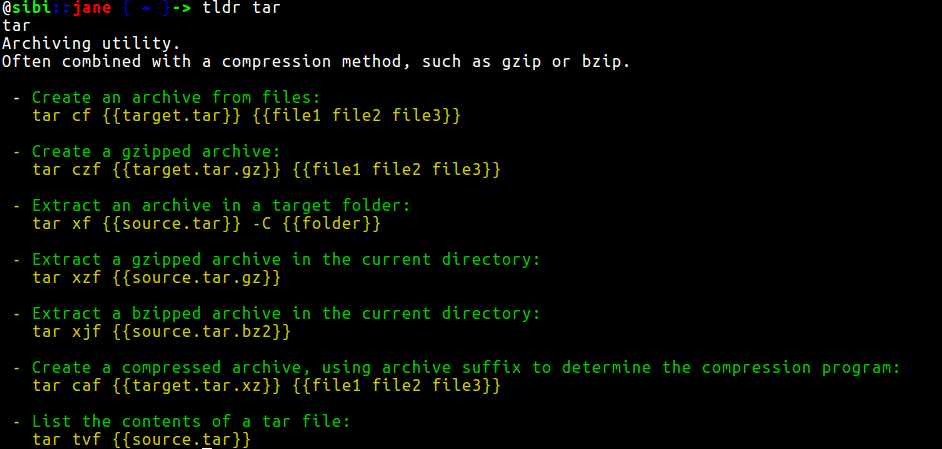
\includegraphics[width=\linewidth]{tldr.png}
  \label{fig:tldr-client}
\end{figure}

Compared to the previous version, the new version does proper
rendering for the edge case scenarios. Also, have added support for
golden testing to avoid regression. Other changes mostly include minor
bug fixes.

\FurtherReading
  \url{https://github.com/psibi/tldr-hs}
\end{hcarentry}

\end{document}
